\documentclass[11pt,a4paper,twoside]{book}

\newcommand{\ficherosBasicosTeXiS}{%
TeXiS/TeXiS_pream,TeXiS/TeXiS_cab,TeXiS/TeXiS_bib,TeXiS/TeXiS_cover%
}
\newcommand{\ficherosBasicosTexto}{%
constantes,Cascaras/bibliografia,config%
}
\newcommand{\compilaCapitulo}[1]{%
\includeonly{\ficherosBasicosTeXiS,\ficherosBasicosTexto,Capitulos/#1}%
}

\newcommand{\compilaApendice}[1]{%
\includeonly{\ficherosBasicosTeXiS,\ficherosBasicosTexto,Apendices/#1}%
}

\include{config}

% Paquete de la plantilla
\usepackage{TeXiS/TeXiS}

\begin{document}

\frontmatter

%---------------------------------------------------------------------
%
%                          configCover.tex
%
%---------------------------------------------------------------------

\tituloPortada{Hunting bugs: Towards an automated approach to identifying which change caused a bug through regression testing}

\autorPortada{Michel Maes Bermejo}

\fechaPublicacion{Septiembre 2023}

\imagenPortada{img/urjc-logo.jpg}
\escalaImagenPortada{.4}

\tipoDocumento{TESIS DOCTORAL}

\institucion{%
Programa de Doctorado en Tecnologías de la Información y las Comunicaciones\\[0.2em]
Escuela Internacional de Doctorado
}

\directorPortada{Micael Gallego Carrillo \\
Francisco Gort\'{a}zar Bellas}

%%
%% Creamos las portadas
%%
\makeCover

%%%
%%% Local Variables:
%%% mode: latex
%%% TeX-master: "../Tesis.tex"
%%% End:


\chapter{Acknowledgements}
\specialHead{Acknowledgements}

Lorem ipsum dolor sit amet, consectetur adipiscing elit. Vivamus faucibus, nunc id accumsan ullamcorper, libero nisi sollicitudin sem, quis porta diam nisl quis nulla. Nam viverra tempor ex eu ultricies. Aliquam at felis sed sapien egestas semper a quis dolor. Maecenas at odio non nibh pulvinar bibendum. In mattis ex et est egestas, iaculis sagittis tellus varius. Cras id posuere lorem. Cras leo risus, sagittis quis ligula ac, vehicula viverra erat. Nam vel iaculis dui, eu ullamcorper felis. Vivamus bibendum purus eget metus sagittis, eu tincidunt dolor hendrerit. Ut porttitor ac lectus eu varius. Class aptent taciti sociosqu ad litora torquent per conubia nostra, per inceptos himenaeos. Maecenas ut blandit metus. Phasellus ut velit ut velit volutpat porttitor.

Orci varius natoque penatibus et magnis dis parturient montes, nascetur ridiculus mus. Cras imperdiet turpis turpis, vitae ultrices risus viverra a. Sed lobortis at enim in venenatis. Aenean porttitor, nunc id tincidunt facilisis, lorem risus laoreet lorem, quis egestas magna mi eget metus. Integer lobortis porttitor nunc, sit amet semper ligula accumsan ut. Etiam blandit erat id tempor auctor. Sed at pulvinar ante. Vestibulum consequat facilisis neque, vel condimentum nisl sodales in. In quis fermentum eros, id dapibus sapien. Etiam hendrerit a urna vitae feugiat.

Mauris condimentum mauris tellus, ut tempus risus feugiat at. Aenean eget ornare nisl, eu gravida libero. Quisque ultricies erat orci, non consectetur dolor laoreet vel. Aenean laoreet sodales turpis vel suscipit. Lorem ipsum dolor sit amet, consectetur adipiscing elit. Ut eu placerat tellus, vel efficitur magna. Praesent ut massa ac quam tristique sollicitudin ac vitae elit. Phasellus id lorem sed est faucibus faucibus id id turpis. Nunc fringilla eros eu sapien placerat faucibus sit amet vitae enim. Etiam sollicitudin iaculis luctus. Nulla facilisi. Integer enim sapien, venenatis vitae mattis vulputate, blandit eu leo. In lobortis erat non augue viverra porttitor sed id justo. Curabitur in dictum lacus, sed malesuada lacus. Aenean sed sapien mi. Proin sit amet nibh ut lectus cursus ullamcorper.

Curabitur finibus est ac quam sagittis, quis porta magna viverra. Aenean nulla enim, sodales vel molestie in, feugiat eu lectus. Duis aliquam consequat urna et efficitur. Vivamus sollicitudin feugiat urna, ut consectetur ex finibus non. Praesent rutrum felis sit amet diam dignissim, at placerat nulla ornare. Integer eget commodo orci, cursus ultricies ante. Nullam consequat iaculis leo nec scelerisque. Etiam eu purus dapibus, hendrerit felis non, pellentesque lorem. Vestibulum in scelerisque quam, et interdum lectus. Proin tellus tortor, vulputate id iaculis sed, consequat a dui. Nulla lacus leo, lobortis vel purus eu, feugiat vestibulum metus. Praesent blandit scelerisque sapien. Fusce sit amet metus erat. Aenean sollicitudin imperdiet pellentesque. Duis volutpat bibendum lacus vel dictum. Ut elementum ullamcorper eros, quis pulvinar lacus.

Aliquam nec viverra nisi, laoreet bibendum ligula. Mauris lorem neque, blandit eu mauris in, porttitor tristique neque. Duis eget ex est. Mauris elementum nunc id semper maximus. Vestibulum lectus diam, ultrices eu nisi et, accumsan pretium eros. Sed pharetra pellentesque nulla, vitae euismod lorem condimentum quis. Quisque non porttitor elit. Sed eleifend iaculis mauris, ac tincidunt elit placerat eget. Phasellus sodales metus a urna convallis, nec auctor sem rhoncus. Morbi egestas finibus ipsum ut scelerisque. Ut sit amet molestie tellus.



\chapter{Abstract}
\specialHead{Abstract}
Finding code changes that introduced bugs is important both for practitioners and researchers, but doing it precisely is a manual, effort-intensive process.
There are several studies that try to automatically detect these changes that introduce the bug. 
The most recognized state of the art in this field is the SZZ, an algorithm based on identifying the change that fix the bug to analyze the lines that have been modified or deleted, assuming that the last change made in those lines before the fix was the change that introduced the bug. 
A recent work (presented as a PhD. Thesis by Gema Rodriguez in 2018) offered a theoretical model, called the "perfect test method", which proposed a completely different approach to the SZZ and aimed to mitigate the limitations of this algorithm. 
The perfect test method is a theoretical construct aimed at detecting bug introducing changes (BIC) through a theoretical perfect test. This perfect test always fails if the bug is present, and passes otherwise.
In theory, this perfect test would allow to detect the bug in the change history of a project.

\patxi{Quizá indicar aquí que los tests de regresión son escritos por los desarrolladores cuando se detecta un bug y se corrige para evitar regresiones, y que al ser una práctica habitual, están disponibles en muchos casos. Esto nos lleva a plantearnos el principal objetivo de la tesis: operacionalizar... basandonos en tests de regresión.}
In this PhD. Thesis, one of the main objectives is to operationalize this theoretical construct. 
This dissertation hypothesizes that regression tests (tests written after finding a bug with the purpose of detecting if it reappears) can be used as perfect tests to detect the change that introduced the bug. 

One of the main problems of operationalizing this approach, pointed out in the previous work, is the difficulty that can be encountered when running this regression test on previous versions of the code. 
A step prior to the execution of the tests is the building of the project, which requires downloading the dependencies of that project and compiling the source code (if the language requires it). 
In order to achieve the above-mentioned objective, this thesis will also carry out a study on the buildability of the previous versions of the code, verifying how far they can be built and what problems can be encountered during the process.
This dissertation also extends the previous\patxi{this study (previous suena a que ya lo han hecho otros)} study to check whether, in addition to being able to build the source code, we can build and run its tests. 
These two studies are intended to shed some light on the problems of the initial proposal in order to be able to implement it with the knowledge acquired.

The results obtained in this thesis show that \patxi{comienza aquí presentando las aportaciones: a) compiling past snapshots is greatly affected by time unless remediation measures are applied; b) testing past snapshots is mainly affected by compilation, but contrary to what was expected, not all tests pass in all commits; c) the operationalization...}the operationalization of the perfect test method through regression tests is feasible and can be completely automated in practice when tests can be transplanted and run in past snapshots of the code. 
Given that implementing regression tests when a bug is fixed is considered a good practice, when developers follow it, they can detect effortlessly bug introducing changes by using the proposed operationalization of the perfect test method.





\setcounter{tocdepth}{2} 

\setcounter{secnumdepth}{3} 

\ifpdf
   \pdfbookmark[1]{Contents}{contents}
\fi

\specialHead{Contents}

\tableofcontents

\newpage 

\specialHead{List of Figures}

\ifpdf
   \pdfbookmark[1]{List of Figures}{List of Figures}
\fi

\listoffigures

\newpage


\ifpdf
   \pdfbookmark[1]{List of Tables}{List of Tables}
\fi

\specialHead{List of Tables}

\listoftables

\newpage

%%%
%%% Local Variables:
%%% mode: latex
%%% TeX-master: "../Tesis.tex"
%%% End:


\mainmatter
\restauraCabecera

\chapter{Introducction}
\label{sec:intro} 
\pagenumbering{arabic}
\section{Motivation}

In software engineering, developers collaborate with each other in order to develop a software product. 
Software developers have been assisted for years by Version Control Systems (VCS). 
These systems have made it possible to manage, coordinate and organize the development of software products. 
During software development, developers implement several changes to the product in order to introduce new functionality or improve pre-existing ones (by means of refactorings or bug-fixings).
These changes can be grouped into a revision, the minimum unit in which a VCS allows us to version our software. 
This revision is also known as a "commit" or "snapshot".
One of the most popular and dominant VCS in recent years has been Git~\cite{VersionControlSystemSurvey:2022:Online}. 
Git was started with the goal of being an open-source distributed version control system for developing the Linux kernel.
Among its main features is its strong support for non-linear development (i.e., multiple users can develop in forked branches of a main branch and then merge the code back together).
%\patxi{No sé si no habría que introducir que puedes tener ramas, que los commits pueden tener uno o varios padres... Esas cosas habría que introducirlas en algún momento. No creo que este sea ese momento, pero habrá que hacerlo para darles más valor del que le dimos en su día en los papers.}
%Git is a distributed version control system that allows developers to work locally and collaborate with other developers.

\patxi{Estos dos párrafos no están muy unidos. Te propongo empezar el segundo así: This version history is fundamental to software evolution and maintenance. Indeed, one of the main activities performed by developers within software evolution and maintenance is bug fixing. ...}
Within software evolution and maintenance, one of the main activities performed by developers is bug fixing. 
These bugs were, at that moment, changes introduced in the change history as commits.
The fixes to these bugs are made through changes that are also reflected in the VCS as a fix commit. 
In other words, both the changes that introduced the bug and the one that fixed the bug are recorded in the VCS. 
From this premise, proposals have emerged to be able to locate the change that introduced the bug from the change that fixed it. 
If the users of our software use different versions of the software, being able to detect which change introduced the bug allows us to understand the scope of that bug and which versions have been affected and therefore should be fixed.
One of the most relevant proposals for locating the change that introduced the bug is the SZZ algorithm~\cite{Sliwerski:2005:CIF:1083142.1083147}. 
This algorithm starts from the assumption that the same lines of code that were modified or deleted in the fix changes are the ones that contained the bug. 
In this way, the change history of a software project could be used to search for the change that introduced or modified those lines and thus be able to know which versions of the project are affected by the bug.

The SZZ algorithm has been for many years the state of the art when locating the change that induced a bug. 
In 2018, Gema Rodriguez presented her PhD. Thesis~\cite{rodriguez2018towards}, in which she exposed the limitations of this algorithm and all those that have been derived from it, finding several examples in which this algorithm failed in its purpose. 
In her research and as part of her thesis, the author proposed a theoretical model for the identification of the change that introduced a bug, trying to improve the state of the art. 
This model, in essence, was based on the idea of the "perfect test", a theoretical construct that was able to check if a bug was present or not in commits prior to the change that fixed it. The author of this work explained the difficulties in operationalizing this theoretical model. 
Among the limitations encountered, she points out the difficulty of finding a candidate to be the "perfect test", the impossibility of compiling some code revisions in the past, or the impossibility of executing code of the present (the perfect test) in the commits of the past.

The motivation of my\patxi{this} PhD. Thesis is to deal with these limitations, to acquire empirical knowledge of the proposed problems and to operationalize the perfect test theoretical model

\section{Hypothesis}

In software projects, there is a common practice that when a bug is detected, not only it is fixed but also a test is implemented to verify that the bug does not reappear (also known as regression testing). 
That bug may have had different life cycles. 
For example, it is possible that the bug has always existed in the code, since the first day the functionality was implemented. 
On the other hand, it is also possible that the bug was a regression, in which case, at some point in the project life cycle, the bug did not exist and was somehow incorporated into the code. 

Our hypothesis is that the tests implemented when the bug is fixed can be used to determine whether the bug was a regression and used as the operationalization of the "perfect test" defined in the theoretical model of the previous work. 
It would be enough to run this test with previous versions of the code. 
If a version is found in which the test passes, then in that version the bug did not exist, and therefore it has been a regression. 
If no previous version is found in which the test passes, then the bug is not a regression, because the functionality never worked correctly, or at least not exactly as verified by the test.

\section{Objectives}

The primary objective of this PhD. Thesis is to validate the hypothesis proposed in the previous subsection, aiming to put into practice the theoretical model proposed in the literature and described in the introduction. \patxi{described here (ya estás en la introducción)}
From the limitations pointed out by the authors of this model, particular objectives arise, related to study the history of the projects in order to understand the feasibility of our proposal.

The objectives of the thesis will be three and correspond to three research projects that complement each other:

\begin{itemize}
    \item To verify the extent to which it is possible to build past commits of a project. To be able to carry out the execution of tests in the past it is required to fulfill the precondition that this code can be built: which means that its dependencies can be downloaded and the code compiles (if the language requires it). 
    There is previous work on this topic that we aim to validate and extend.
    \item To verify the extent to which it is possible to run the tests in the past. This objective extends the purpose of the previous one, extending it by means of trying to execute the tests after the code was compiled. As there is no previous work on this topic (at the time of writing this thesis), we aim to propose new metrics that will help us to assess the project level coverage provided by the tests.
    \item To apply the knowledge acquired in achieving the previous objectives to \patxi{verify our hypothesis: that it is possible...}solve our initial objective: to validate the hypothesis that it is possible to use regression testing as a "perfect test" following the theoretical model proposed in the literature.
    For that purpose, we will run regression tests along the commit history of the project to detect the change that introduced the bug.
\end{itemize}

\section{Contributions}

The main contributions of this thesis are outlined below.
These contributions will be detailed in the corresponding chapters.

\begin{itemize}
    \item \textbf{A replication and a reproduction study of the compilability of the history of past commits of a project}
    This contribution addresses the first objective defined in the previous section.
    It is a research study that investigates about the compilability of the history of past commits of a project.
    This research is conducted through a replication of a previous study~\cite{tufano2017there} (using the original set of real software projects from that study) and a replication (using a new set of projects).
    This contribution has been published in the Empirical Software Engineering journal in March 2022~\cite{maes2022revisiting}.
    \item \textbf{A study of the testability of the history of past commits of a project}
    This contribution addresses the second objective defined in the previous section.
    This research proposes a case study where new metrics are discussed to measure how testable the change history of a project is. It also offers an analysis of the results of these metrics for a well-known project dataset.
    This contribution is planned to be submitted at the Software Evolution and Process journal.
    \item \textbf{An empirical method for detecting the change that introduced a bug through regression tests}
    This contribution addresses the third objective defined in the previous section. 
    This study proposes the operationalization of a previous theoretical model, in which our proposal offers a tool to automatically detect the change that introduced the bug using regression tests. 
    To accomplish this, we will start from a well-known dataset of software projects that have labeled the changes that fix a bug together with a regression test that reveals that bug.
    This contribution has been submitted to Empirical Software Engineering journal and is under review at the time of this writing.
    % \item{Otros} \michel{Si hay tiempo, podemos añadir otros artículos relacionados: el dataset de regressiones e2e y su continuación, la identificación de proyectos e2e en GitHub}
\end{itemize}

\section{Organization of the thesis}

The remainder of this thesis is organized as follows.
In Chapter~\ref{chapter:related-work} we present the related work to the reader. 
Section~\ref{sec:buildability:related} discusses previous studies on software compilability. 
Section~\ref{sec:testability:related} discusses previous studies on software testability. 
Section~\ref{sec:transplating-code:related} details how other authors have approached transplanting code. 
Section~\ref{sec:bic:related} introduces the state of the art in the detection of the change that introduced a bug.
Chapter~\ref{chapter:buildability} addresses the study on software compilability, corresponding to the first contribution of the thesis.
Chapter~\ref{chapter:testability} addresses the study on software testability, corresponding to the second contribution of the thesis.
Chapter~\ref{chapter:bug-hunter} addresses the study on the detection of the change that introduced a bug, corresponding to the third contribution of the thesis.
Finally, Chapter~\ref{chapter:conclusions} draws the conclusions and outlines the future work.
 

\chapter{Related work}
\label{sec:related}
Probably the most relevant research on build errors is the empirical study by Seo et al.~\cite{Seo:2014:PBE:2568225.2568255} that examined over 26.6 million builds triggered in Google's centralized build environment.
An error taxonomy was provided by this study based on log patterns.
%\grex{What differs or adds our work in comparison to this one?}
Sulir and Porub\"an examine the builds of more than 7000 Java projects, but only for their last commit~\cite{Sulir:2016:QSJ:3001878.3001882}.
In both studies, they have performed a study \emph{in amplitude}.
Compared to them, in this this work, we will limit the number of projects to study all their history -- our effort can thus be considered a study in depth.

Rausch et al.~\cite{Rausch:2017:EAB:3104188.3104231} address the reasons why builds fail in the context of Continuous Integration (CI) environments.
These authors extracted outputs from Travis (a CI tool) from 14 open-source projects, along with information from their public Git repositories.
An important percentage of error outputs correspond to the tests that have not passed, but they give special importance to the cases where the failed build previous to the tests is the cause of the error.
In addition to categorize the main errors found by the CI system, they also consider other metrics (e.g., number of authors, number of lines modified, frequency of changes, among others).
The study contemplates the analysis of the history of the builds from the approach of continuous integration (construction of the project together with the tests).
Our approach tries to verify what would happen if instead of taking the outputs of CI, we execute ourselves the build of the project (not considering tests) to check if all commits are able to be built (i.e., if the commit is buildable).
Rausch et al.'s study is limited to the builds made by the CI, which do not correspond to the number of commits of the project.
%It is therefore a line to approach to check if all the commits of a project can be built.

Buildability may have a huge impact on those areas where building past commits of the project is key.
This is the case for bug localization~\cite{Sliwerski:2005:CIF:1083142.1083147,Asaduzzaman:2012:BIC:2664446.2664463, Murgia:2010:MLA:1852786.1852794, Zimmermann:2006:MVA:1137983.1138001, Zimmermann2008}.
When localizing bugs, techniques like git bisect may be used to traverse the project history of commits back to the past in order to find the set of lines in a commit that introduced a bug~\cite{spinellis2012git, meneely2013patch}.

Some authors have emphasized the importance of historical versions to propose repair tools of failed builds~\cite{HireBuild}, or have proposed metrics to evaluate the stability of the project over time~\cite{6405296}.
Others have addressed the problem in an indirect way.
For instance, Just et al. found this problem when trying to run mutant tests in previous versions of several software projects~\cite{Just:2014:MVS:2635868.2635929} provided by Defects4J~\cite{Just:2014:DDE:2610384.2628055}.

Reproducibility of research is a popular topic of interest among researchers to validate findings from other publications~\cite{RODRIGUEZPEREZ2018164} and projects~\cite{4693714}.
Although much attention has been put on the availability of publicly available datasets (e.g., datasets on defect prediction~\cite{wahono2015systematic}), the software developed and used by researchers has shown to have major importance~\cite{rodriguez2012software, bruntink2014initial}.
The software engineering research community has proposed some solutions that facilitate scientific software reproducibility in the future~\cite{DBLP:journals/corr/Weber17,DockerReproducibility2016,Boettiger:2015:IDR:2723872.2723882}.

%The reproducibility of experiments in software engineering is a subject widely discussed by Juristo et al.~\cite{juristo2004improving,juristo2011role,gomez2014understanding}.


%\grex{We have to mention Juristo's work in empirical software engineering on reproducing experiments}

%Gonz{\'a}lez-Barahona and Robles note that ``reproducibility of experiments is one of the basic rules in the scientific method''~\cite{González-Barahona2012}.


As pointed out in the introduction, a term related to buildability and very recurrent recently is build reproducibility.
%buildability is the first step to achieve reproducibility and therefore the focus of our research.
%Build reproducibility is the ability to generate byte-to-byte identical binaries from the source code of the project, at any point of its history, no matter who builds the binary, when or in which machine~\cite{RepBldsDebian:2018:Online}.
%Some authors also include test in build process.
Software distributors, such as the Debian community, have a strong interest in the reproducibility of builds~\cite{RepBlds:2017:Online,RepBldsDebian:2018:Online}.
Ren et al. focus on reproducible builds in Debian packages~\cite{Ren:2018:ALU:3180155.3180224}.
In it, the authors present a framework for detecting and fixing reproducible problems in Debian packages, but they focus exclusively on the latest commit, and they do not analyze the reproducibility of those packages in the past.
Glukhova also discusses the reproducibility of Debian packages by offering tools that ensure reproducibility~\cite{Glukhova:Thesis:2017}.
The reproducibility of builds is also interesting from a security point of view.
Some works focus on bringing security into the software development life cycle, and they mention build reproducibility as one of the main issues to be taken into account.
De Carn\'e de Carnavalet and Mannan mention the use of reproducible builds in the context of security-critical open source software~\cite{deCarnedeCarnavalet:2014:CIV:2664243.2664288}.
Nikitin et al. propose a decentralized software-update framework that includes build verifiers to validate the source-to-binary correspondence~\cite{nikitin2017chainiac}.
Al-Bassam and Meiklejohn propose a system to ensure binary transparency~\cite{10.1007/978-3-030-00305-0_8}.
Skrimstad noted about the trust in software through reproducible builds~\cite{Skrimstad:Thesis:2018}.

Build reproducibility is typically studied in stable versions of the project where a binary is available.
We are interested in building not only the stable versions, but all project snapshots for which there is usually not binary, which allows to be used in scenarios such as bug fixing, among others.
Thus, while a software project requires to meet additional criteria to achieve build reproducibility than to be buildable, complete historic buildability demands a software project to have many more snapshots to be buildable.

%In comparison, our work addresses all versions (releases, betas and snapshots), instead of just the latest stable version.

%\grex{You say there is just one work, but then refer to two}

%\grex{A good idea here would be to tell how our approach differs from what has been previously done.}





\chapter{Methodology}
\label{sec:metodology}
Our objective is to analyze multiple projects, checking whether we can build  or not every snapshot.
For those snapshots whose build fails, we study the build logs to determine which are the most common errors that prevent a snapshot from being buildable, grouping and categorizing errors in a taxonomy.

%Reproducibility is a topic of interest among researchers to validate other publications~\cite{RODRIGUEZPEREZ2018164} and projects~\cite{4693714} through reproducibility, in addition to offering solutions that facilitate reproducibility in the future~\cite{DBLP:journals/corr/Weber17,DockerReproducibility2016,Boettiger:2015:IDR:2723872.2723882}. For this reason,
 
We have tried to make our experiment reproducible so that any researcher can obtain the same results as we do or use our data for other investigations.
The reproducibility package for this work can be found in a public repository\footnote{\url{https://github.com/Maes95/TFM-Buildability/tree/ReproducePackage/Tools}}.

%\mica{New section to discuss reproducibility of the project?}
%\grex{This belongs to the methodology section and should be better a footnote with the URL, not a cite.}

\section{Subject programs}

To choose what projects are suitable for this study, we consider some desirable characteristics that make them easy to build:

\begin{itemize}
	\item Using a compiled language (e.g., Java or C++), so that when developing, type-safety is enforced during the build phase, avoiding type problems in runtime.
In addition, we can obtain more information at the build phase than from projects using a dynamic language.
	\item Project dependencies are simple to obtain, for example, from a remote repository.
	\item The environment in which the project was built is easy to set up, or has no impact on the build.
\end{itemize}

Following Easterbrook \emph{et al.}~\cite{easterbrook2008selecting}, we selected six exploratory case studies to gain a deep understanding of the buildability in six open source projects.
For this purpose, we selected projects written in Java, a static typed programming language that is platform-independent, with a freely available compiler.
Java has also backward compatibility and multiple tools to manage dependencies like Maven, Gradle or Ant.
In order to study the buildability of a project, the history of the projects needs to be available through some source control management (SCM) system.
The selected projects are available in Git repositories, so we used Git to traverse their history.

Table~\ref{table:projects} shows the six open source Java projects selected for the study.
For each project, we display the number of snapshots (commits) that are available in their respective git repositories, and the build system used by the project to compile the source code and generate the binaries.
Five projects come from a common dataset in software research, Defects4J~\cite{Just:2014:DDE:2610384.2628055}.
These projects are commonly used for research in Software Testing.
It is important to note that they are small projects with a limited set of dependencies.
The only exception is the Closure project, with 12 dependencies, which are included in the source code without the need to recover them from an external repository.

%\grex{Could we have the number of dependencies as well? As I suppose they vary over time, it would be good to provide a range of the number of dependencies.}
To expand our dataset, we also analyze the Spring Framework project.
This project is a large multi-module project, widely used in the industry for developing Java web applications.
The complexity of this project is far beyond that of the Defects4J projects.
It has as well a higher number of dependencies.

\begin{savenotes}
	\begin{table}
		\caption{Projects used in this work}
		\label{table:projects}
		\centering
		\begin{tabular}{crcr}
			\toprule
			\bf{Project} & \bf{\# Snapshots} & \bf{{Build system}} & \bf{\# Dependencies}\\ 
			\midrule
			Closure Compiler & 2,858 & Ant & 12\footnote{Dependencies are in source files}\\
			Commons-lang & 3,570 & Maven & 3\\
			Commons-math & 4,878 & Maven & 1\\
			Mockito & 2,639 & Gradle & 4\\
			Joda-Time & 1,717 & Maven & 2\\
			Spring Framework & 17,382 & Gradle & 20\footnote{Optional dependencies are not counted}\\
			\bottomrule
		\end{tabular}
	
	\end{table}
\end{savenotes}

\section{Analysis process}

The analysis consisted in two phases, a first one for checking buildability of the project (\textit{Check build process}), and a second one for analyzing the data collected of the failed builds (\textit{Log analysis}) in order to perform the classification.

%\grex{I don't know if ``experiment'' is the right wording}

\subsection{Check build process}

This process is shown in Figure~\ref{fig:commitHist}.
It starts with the most recent commit of the project.
This commit is checked out, and the project is built from its source files using the appropriate build system for the project (as defined in Table~\ref{table:projects}).
To determine the build status, we check the exit code of the build process: zero signifies success, and non-zero signifies failure.
If the build succeeds, it is marked as success.
Otherwise, it is marked as failure and the logs generated during the build process are saved for later inspection.
Then we go back to the previous commit, and repeat the whole process.
This process is repeated until we reach the first commit in the repository.
Figure~\ref{fig:commitHist} summarizes the process in a visual form.

% \begin{figure}[h]
% 	\centering    
% 	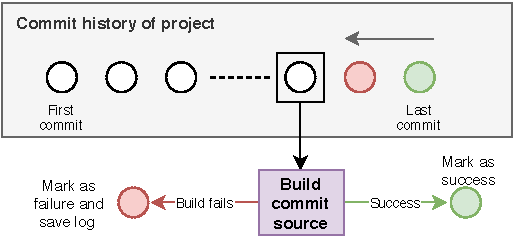
\includegraphics[width=12cm]{img/CommitHist.pdf}
% 	\caption{Check build process}
% 	\label{fig:commitHist}
% \end{figure}

Due to the large number of commits in the history of the selected projects, building them manually is not practical.
In order to automate the process, we developed a Python script that given a configuration file, a build script and the git project, basically executes the process described above iteratively for each commit.
To build each project, the basic commands of each construction tool have been used, taking into account the documentation of each project (e.g., a Maven build is shown in Listing~\ref{listing:mvnscrpt}).
In most projects, it is important to clean the output folders to avoid reusing files when changing between commits.
To reproduce these steps in a simple way without having to worry about the environment or the necessary technologies, this execution is encapsulated in a Docker\footnote{https://www.docker.com} container.

%\mica{Ampliar esto mencionando que incluye este paquete}

%\grex{I would like to hear something about the dependencies here...I remember hearing from Michel that he set up an environment where he run the experiment... please, include that info here!}

\begin{lstlisting}[caption={Example of a Maven build command},captionpos=b, label={listing:mvnscrpt}]
                      mvn clean install -Dmaven.test.skip=true
\end{lstlisting}


\subsection{Log analysis} 
\label{sssec:logAnalysis}

Our analysis (depicted in Figure~\ref{fig:AnalysisProcess}) takes as input:
   i) the commit history of the project (where each commit is marked as success or failure), and
   ii) the logs for the commits marked as a failure.
Our aim is to perform an analysis of the logs to determine the reasons why the build failed.

% \begin{figure}[h]
% 	\centering    
% 	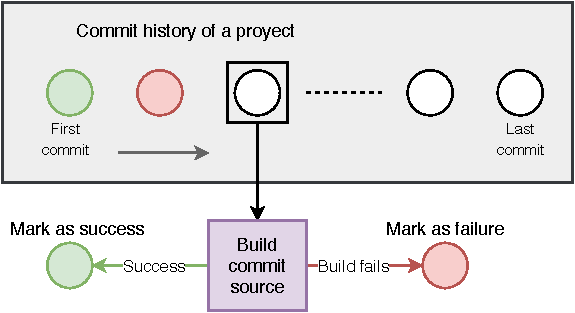
\includegraphics[width=12cm]{img/AnalysisProcess.pdf}
% 	\caption{Analysis process for builds that fail.}
% 	\label{fig:AnalysisProcess}
% \end{figure}

We assume that consecutive commits which fail between two successful commits are likely to contain the same error.
Based on this idea, choosing a log from a group of consecutive commits, we can extract the error trace that identifies the problem and generate a pattern from it.
Once we have a consistent number of patterns, we apply them in order (from more specific to more generic) to each log, stopping when a match occurs, continuing with the next log.
This process is iterative: new patterns are generated to eliminate very generic patterns and group the logs better.
We finish the process when all logs match a pattern and can be grouped without confusion.

We will call this error trace a \textbf{symptom}.
We then group similar patterns together, in order to identify those logs that share the same symptom.
For each symptom that we find, a \textbf{cause} (i.e., the error that causes the symptom) can potentially be attributed to it.
The cause, in many cases and due to the Java logging system, can be extracted together with the symptom.
In other cases, the cause is more ambiguous and requires interpreting the log along with the failed version of the project, exploring it in detail (sometimes at a very low-level).
In a next step, our intention is to categorize the error according to its nature using a method for taxonomy development.

%Once the cause is determined, we assess \textbf{if the error could be solved} by applying a change -- or if it is unsolvable.
%In case it is solvable, it is necessary to determine if it needs a) a simple change (e.g., adding a trivial script during the build) or b) a major change is necessary (e.g., a non-trivial modification of the source code).
%\michel{We should mantain this? We have no solutions for the errors}

To clarify the process, we present a didactic example is shown in Listing~\ref{listing:pattern}.
In this case, an error pattern is applied to the log obtained after a failed execution in the Spring Framework.

% \textcolor{black}{Pattern: }
\begin{center}
	\begin{lstlisting}[linewidth=\linewidth, caption={SpringFramework Log - Commit 8961}, captionpos=b, label={listing:pattern}]
	<@\textbf{Pattern: }@><@\textbf{\textcolor{violet}{Could not find (.+)}}@>
	<@\textbf{Log with pattern matching: }@>
	FAILURE: Build failed with an exception.
	
	* What went wrong:
	Could not resolve all dependencies for configuration ':spring-messaging:optional'.
	> <@\textbf{\textcolor{violet}{Could not find org.projectreactor:reactor-net:1.1.0.BUILD-SNAPSHOT.}}@>
	Required by:
	org.springframework:spring-messaging:4.1.0.BUILD-SNAPSHOT
	\end{lstlisting}
\end{center}


\begin{itemize}
	\item \textbf{{Symptom}}: The trace highlighted in the log can not resolve a dependency.
	\item \textbf{{Cause}}: An unspecified development (BUILD-SNAPSHOT) version is used and can not be recovered.
	%\item \textbf{{Could be solved?}}: It is resolvable, apparently easy, replacing the version with a stable one (release)
\end{itemize}



%\grex{I think it would be very didactic to show an example of an error log, to highlight where we see that we can find the cause. Doing this with an example, including a code excerpt would make the methodology easier to follow.}

Most of this process is automated.
We use Jupyter notebooks to make the interaction with the data more versatile.
We define the patterns by means of regular expressions (see Table~\ref{table:commmonErrors} for some examples).
Then, we count the number of occurrences of each pattern in the history of builds for the six projects under study.

\begin{table}
	\caption{Some common error patterns for Java projects}
	\label{table:commmonErrors}
	\begin{center}
		\begin{tabular}{c}
			\toprule
			\verb|error: (.+)\n(.+)| \\
			\midrule
			\verb=(> Could not resolve|> Could not find) (.+)= \\
			\midrule
			\verb|unable to resolve class (.+)| \\
			\midrule
			\verb|Exception in thread (.+)| \\
			\bottomrule
		\end{tabular}
	\end{center}
\end{table}

\section{Taxonomy development}\label{subsec:taxonomy}

The development of taxonomies is not limited only to software engineering, it has its origin in other fields such as biology~\cite{eldredge1980phylogenetic,sneath1973numerical} or Social Sciences~\cite{bailey1994typologies}.
The development of a taxonomy is not an easy task and requires to search a method that allows us to rigorously address the problem.
For the development of our taxonomy, we base ourselves on the well-known work by Nickerson, Varshney and Muntermann from the field of Information Systems~\cite{Nickerson2013}.
They propose a method to approach the creation of a taxonomy, which has been widely used by other researchers, e.g.~\cite{Krug2012APT,Geiger2011ManagingTC}.
The method is based on the fact that a taxonomy is a set of dimensions, each consisting of mutually exclusive and collectively exhaustive characteristics.
Therefore, each object that we want to classify will take a characteristic in each dimension.
The method allows us to combine both empirical-to-deductive and deductive-to-empirical approaches to identify the dimensions and corresponding characteristics.

In our case, the objects to be classified to obtain the taxonomy will be the causes, using the symptoms to classify them.
The classification will be done iteratively, using in each iteration a portion of the sample of symptoms obtained.
The ending condition will be that all the symptoms obtained have been classified, in addition to the objective ending conditions that the method defines.





\chapter{Computer description}
\label{sec:compdesc}
\section{Development tools}

\subsection{Docker} 

Docker~\footnote{\url{https://www.docker.com}} is an open source software platform to create, deploy and manage virtualized application containers on a common operating system. Docker uses resource isolation features of the Linux kernel (like cgroups and namespaces), to allow containers to run within a single instance of Linux, avoiding the overload of starting and maintaining virtual machines. We will use a docker to ensure that the experiment carried out can be reproduced in a simple way and obtain the same results.

\subsection{Anaconda}

Anaconda~\footnote{\url{https://www.anaconda.com/}} is a free and open distribution of Python and R languages, used in data science, machine learning and Big Data. We use this tool to manage the Python interpreter for the scripts that automate the tasks of the experiment inside a Docker container. In addition, it allows us to use Jupyter Notebook, an interactive tool for the browser that allows us to work easily with the data from the experiments.

\section{Design and Implementation}

In order to implement the process described in Chapter~\ref{sec:metodology} (Analysis process), the technologies presented above (Docker and Anaconda) have been used to build a Docker container with everything necessary to execute the experiment. 

The structure of the folders is as follows:

\begin{itemize}
	\item \textit{analysis/} Folder shared between the host and the container where the results are stored.
	\item \textit{configFiles/} Folder that includes the configuration of the execution of each project and its execution script.
	\item \textit{proyects/} Folder that includes the projects to be analyzed as Git repositories, navigable throughout their commits history.
	\item \textit{py/} Folder that includes Python scripts that provide the logic to execute all the project history builds and store the results.
\end{itemize} 

% \begin{figure}[h!]
% 	\begin{center}
% 		\includegraphics[width=16cm]{img/AppDiagram}
% 		\caption{Project structure}
% 		\label{fig:app}
% 	\end{center}
% \end{figure}

Figure~\ref{fig:app} shows the structure of the tool built to carry out the experiment.

Inside the container and in order to execute the \textbf{Check Build} phase, the following steps are followed:
\begin{enumerate}
	\item Python script $checkBuildHistory.py$ is launched, which will take the configuration file of a project together with its construction script.
	\item The construction of the project is executed from the source code provided in the commit N.
	\item The produced logs are stored, as well as the exit code of the construction process.
	\item Repeat steps 2 and 3 until N=0 (the first commit of the project) is reached.
\end{enumerate}

To approach the \textbf{Log Analysis} phase, we will use Jupyter Notebook to interact with the data in a simple way. This tool will take the logs and exit codes of each commit, selecting those that have failed to make a grouping of the logs. Figure~\ref{fig:jupyter} shows a fragment of these notebooks where the frequency of the errors found in the failed builds of the Spring Framework project is obtained. 

% \begin{figure}[h!]
% 	\begin{center}
% 		\includegraphics[width=14cm]{img/Jupyter}
% 		\caption{Screenshot of Jupyter Notebook - Log analysis for Spring Framework}
% 		\label{fig:jupyter}
% 	\end{center}
% \end{figure}




\chapter{Experimental results of the projects analysis}
\label{sec:results}
In this chapter, we will address RQ1 based on the results obtained for each project.
The results will be shown visually using a \emph{historical graph}, a graphic representation that allows to easily identify the timespan for which commits we could built or not.
In addition, we will group the errors obtained from the logs when commits could not be built.

A summary with the results is shown in Table~\ref{table:allResults}.
This table offers, for each project, the total number of commits available in its history, the number of commits whose build succeeded, the number of commits whose build failed, the percentage of failures with respect to the total of commits, and the number of distinct syntoms (result of grouping identical errors).We can see that there is a project with hardly any errors (Closure Compiler). With the exception of the Apache Commons-math project, in the remaining projects, the failure rate exceeds 40\%. The Spring Framework project stands out not only for its size (it has a multitude of modules) and for its large number of commits, it also has a great variety of different symptoms detected that considerably enrich the later taxonomy.
The rest of this chapter presents a more detailed analysis for each of the projects.

\begin{table*}[h]
	\caption{Summary of experiments}
	\label{table:allResults}
	\begin{center}
	\begin{tabular}{crrrrr}
		\toprule
		\bf{Project} & \bf{\# commits} & \bf{\# success} & \bf{\# fails} & \bf{\% fail} & \bf{\# distinct syntoms}\\ 
		\midrule
		Closure Compiler & 2,858 & 2,855 & 3 & 0.10\% & 3\\
		Apache commons-lang & 3,570 & 1,897 & 1,673 & 46.86\% & 14\\
		Apache commons-math & 4,878 & 3,858 & 1,020 & 20.91\% & 18 \\
		Mockito & 2,639 & 538 & 2,101 & 79.61\% & 9 \\
		Joda-Time & 1,717 & 224 & 1,493 & 86.95\% & 1 \\
		Spring Framework & 17,382 & 6,013 & 11,070 & 63.68\% & 41\\
		\midrule
		Average & 5,507.3 & 2,524 & 2,983.3 & 50.20\% & 14,3 \\
		\bottomrule
	\end{tabular}
	\end{center}
\end{table*}

\section{Closure Compiler}

Our results show that the Closure Compiler project is a highly buildable project (Figure~\ref{fig:closureHist}) with 2,855 commits that can be built out of 2,858 (only 0.1\% of the builds failed).
Note that in the figure older commits appear on the left, with more recent commits on the right.
%Each column in the graph represents 100 commits. \grex{Maybe we should explain a little bit more the graph... I don't understand for instance why we have the white square for the most recent commits}\michel{An explanation of the graphics prior to the individual studies?}
Users of this project can rely on almost any previous snapshots being \emph{buildable}.
%The errors that occur are residual.

\begin{figure}[h]
	\begin{center}
		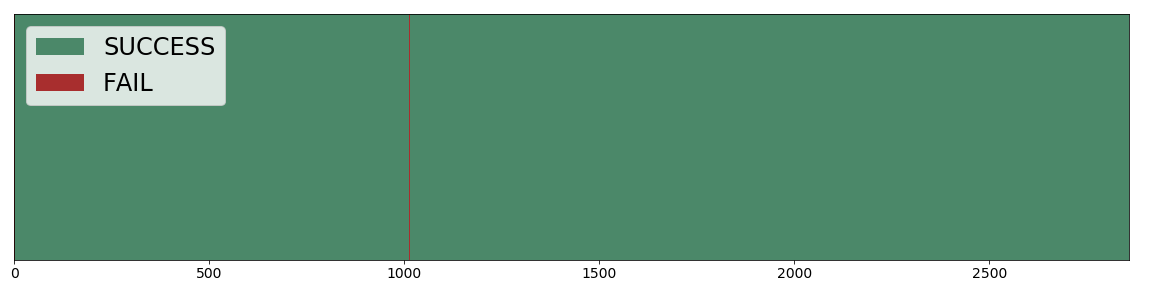
\includegraphics[width=\linewidth]{img/charts/ClosureHist}
		\caption{Build history of Closure Compiler project}
		\label{fig:closureHist}
	\end{center}
\end{figure}

\section{Apache commons-lang}

\begin{table}[h]
	\caption{Grouped errors in Commons-lang builds}
	\label{table:langErrors}
	\begin{center}
	\begin{tabular}{lr}
		\toprule
		\bf{Error} & \bf{count} \\ 
		\midrule
		There is no POM in this directory & 1,524 \\
		Unmappable character for encoding UTF8	& 110 \\
		error: cannot find symbol in NullComparator.java & 20 \\
		Non-resolvable parent POM & 5 \\
		error: cannot find symbol in UnicodeUnescaper.java & 2 \\
		IDKey is not public in org.apache.commons.lang & 2 \\
		Error: variable options might not have been initialized & 2 \\
		Error: incompatible types & 2 \\
		Others & 6 \\
		\bottomrule
	\end{tabular}
	\end{center}
\end{table}

%\grex{I see some of the errors begin with ``Error: '', others don't. Could we have families of higher-level errors?}

In this project we can observe a consistent build failure starting around the middle of the history (Figure~\ref{fig:langHist}).
In this case, we obtain a failure rate that reaches almost half of the project (46.86\%).
The errors collected for this project are shown in Table~\ref{table:langErrors}.

\begin{figure}[h]
	\begin{center}
		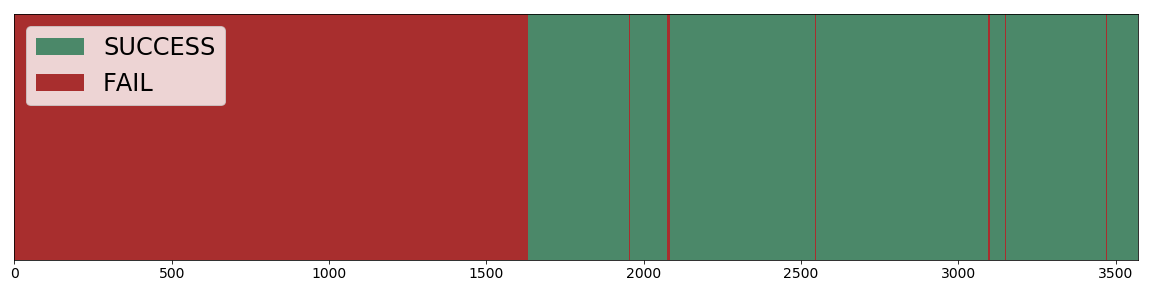
\includegraphics[width=\linewidth]{img/charts/LangHist}
		\caption{Build history of Apache Commons-lang project}
		\label{fig:langHist}
	\end{center}
\end{figure}

The main error of this project is the absence of the \textit{pom.xml} \emph{config} file, which is used by the maven build system to build the application.
When we looked into this, it was clear that this happened because the build system changed at some point; the project stopped using Ant to start using Maven.

\section{Apache commons-math}

The Math project is a robust one (Figure~\ref{fig:mathHist}), with a low failure rate (20.91\%).
Similar to the commons-lang project, there is a specific commit from which the builds begin to fail.
The errors collected are shown in Table~\ref{table:mathErrors}.

\begin{figure}[h]
	\begin{center}
		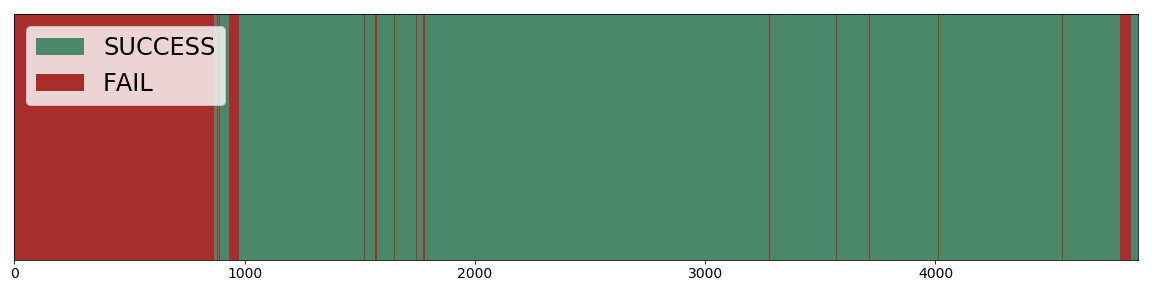
\includegraphics[width=\linewidth]{img/charts/MathHist}
		\caption{Build history of Apache Commons-math project}
		\label{fig:mathHist}
	\end{center}
\end{figure}


As in the Lang project, the build system for the project was changed, from Ant to Maven, which causes any build to fail in the most recent commits of the project.

\begin{table}[h]
	\caption{Grouped errors in Commons-math builds}
	\label{table:mathErrors}
	\begin{center}
	\begin{tabular}{lr}
		\toprule
		\bf{Error} & \bf{count} \\ 
		\midrule
		Can't read pom.xml: No such file or directory & 866 \\
		Failed to execute goal jacoco-maven-plugin & 52 \\
		Failed to execute goal cobertura-maven-plugin & 43 \\
		Error: cannot find symbol & 28 \\
		Failed to execute goal maven-compiler-plugin & 10 \\
		error: no suitable method found & 4 \\
		error: data has private access in ArrayFieldVector & 2 \\
		error: cannot assign a value to final variable entries & 2 \\
		error: Java name clash, have the same erasure & 2 \\
		error: SparseRealMatrix is not abstract & 2 \\
		error: LUDecompositionImpl is not abstract & 2 \\
		Others & 7 \\
		\bottomrule
	\end{tabular}
	\end{center}
\end{table}

\section{Mockito}

This project shows a very low buildability.
Most of its history commits (see Figure~\ref{fig:mockitoHist}) cannot be built.

\begin{figure}[h]
	\begin{center}
		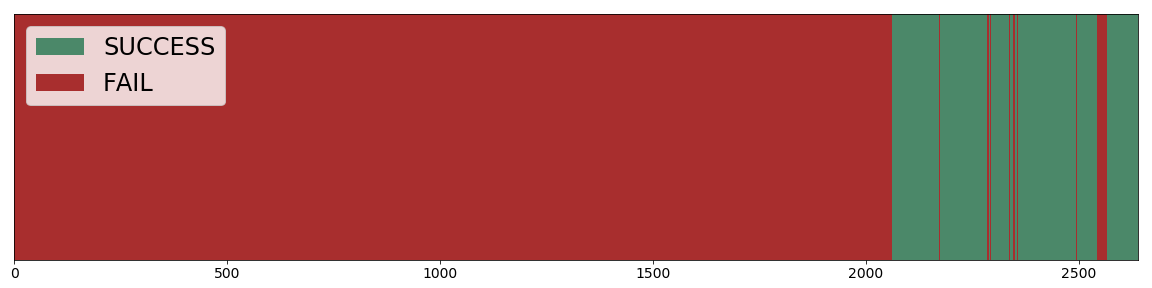
\includegraphics[width=\linewidth]{img/charts/MockitoHist}
		\caption{Build history of Mockito project}
		\label{fig:mockitoHist}
	\end{center}
\end{figure}

\begin{table}
	\caption{Grouped errors in Mockito builds}
	\label{table:mockitoErrors}
	\begin{center}
	\begin{tabular}{lr}
		\toprule
		\bf{Error} & \bf{count} \\ 
		\midrule
			gradlew: No such file or directory & 1,622 \\
			can't read buildSrc/build.gradle: No such file or directory & 440 \\
			Could not find net.bytebuddy:byte-buddy:0.2.0. & 14 \\
			A problem occurred evaluating script & 9 \\
			Execution failed for task ':jar'. & 6 \\
			Execution failed for task ':compileGroovy'.& 4 \\
			Execution failed for task ':compileJava'. &	3 \\
			unable to resolve class ReleaseNotesServices & 2 \\
			Others & 1 \\
		\bottomrule
	\end{tabular}
	\end{center}
\end{table}

The analysis of errors (Table~\ref{table:mockitoErrors}) shows that the main error found is that the \emph{gradlew} executable does not exist, due to a change in build system from Ant a Gradle.
Another very repeated error is the non-location of the build.gradle file, that was moved at some point to a different folder.


\section{Joda-time}

In this case (see Figure~\ref{fig:timeHist}), we found a high percentage of failures (86.95\%) that, in all cases, are due to a change of the build system, from Ant to Maven.

\begin{figure}[h]
	\begin{center}
		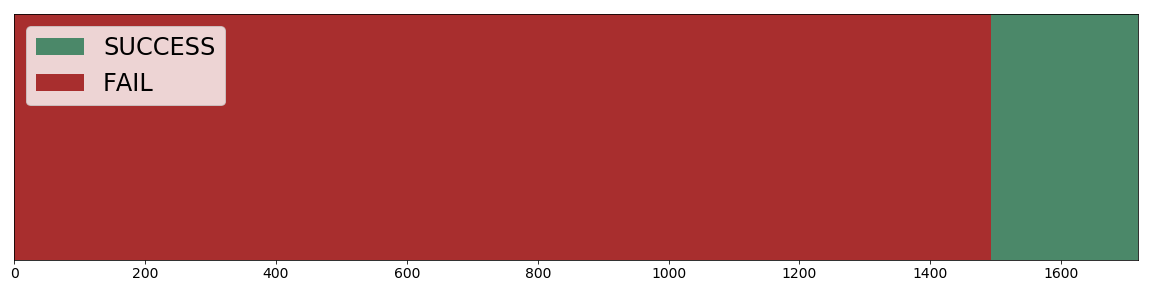
\includegraphics[width=\linewidth]{img/charts/TimeHist}
		\caption{Build history of Joda-time project}
		\label{fig:timeHist}
	\end{center}
\end{figure}

\section{Spring Framework}

This project is, by far, the one that contains more commits, which gives us a broader vision of how a more complex project behaves.
Just over two-thirds of the project's history (as shown in Figure~\ref{fig:springHist}) cannot be built.
There is a consecutive set of commits where it becomes more buildable.
Finally, in the more recent versions of the project, it is again difficult to find buildable commits.

\begin{figure}[h]
	\begin{center}
		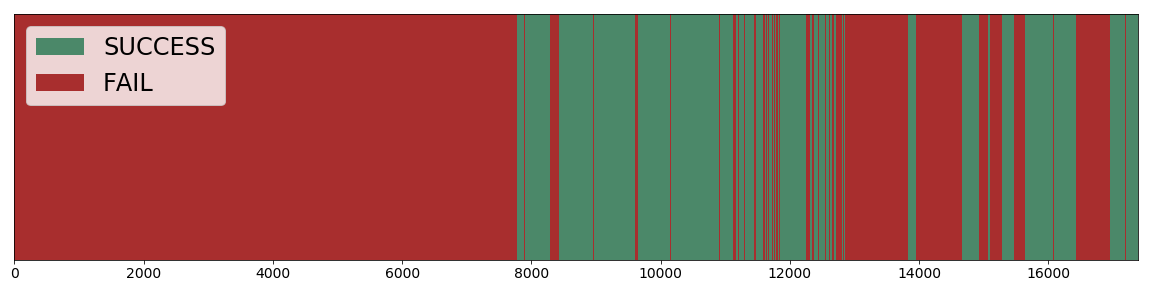
\includegraphics[width=\linewidth]{img/charts/spring-frameworkHist}
		\caption{Build history of Spring Framework project}
		\label{fig:springHist}
	\end{center}
\end{figure}

\begin{table}
	\caption{Grouped errors in Spring Framework builds}
	\label{table:springErrors}
	\begin{center}
	\begin{tabular}{lr}
		\toprule
		\bf{Error} & \bf{count} \\ 
		\midrule
		gradlew: No such file or directory& 5633  \\
		Cannot allocate memory & 2353  \\
		Invalid byte tag in constant pool & 470   \\
		Could not find group:com.itextpdf & 460   \\
		The import java.util.Arrays cannot be resolved & 398   \\
		error: warnings found and -Werror specified 1 error & 328   \\
		Bad file descriptor & 299   \\
		error: cannot find symbol & 218   \\
		error: incompatible types & 210   \\
		Could not determine which tasks to execute  & 206   \\
		error: unmappable character for encoding ASCII  & 202   \\
		Could not resolve all dependencies for spring-webmvc:optional & 132   \\
		error: constructor (..) cannot be applied to given types & 80 \\
		Execution failed for task ':spring-asm:compileJava'. & 77    \\
		error: constructor (..) cannot be applied to given types & 72    \\
		error: EmbeddedDataSourceProxy is not abstract & 64    \\
		FileNotFoundException & 41    \\
		error: package javafx.application does not exist & 28    \\
		Could not resolve all files for configuration ':classpath'. & 25    \\
		Could not find reactor-net:1.1.0.BUILD-SNAPSHOT. & 19    \\
		Could not find reactor-core:1.0.0.BUILD-SNAPSHOT. & 10    \\
		A problem occurred evaluating root project 'spring' & 9 \\
		error: no suitable method found & 6 \\
		A problem occurred evaluating root project 'spring' & 6     \\
		error: local variable (..) is accessed from within inner class & 3     \\
		error: GenericApplicationContext is not abstract & 3     \\                                                                       
		error: invalid method declaration; return type required & 2  \\
		error: package (..) does not exist & 2 \\    
		Others & 10 \\
		\bottomrule
	\end{tabular}
	\end{center}
\end{table}

As can be seen in Table \ref{table:springErrors}, the number of different errors for this project is far above any other of the studied projects.
The most common error is once again due to a change in the build system, from Ant to Gradle.
Other problems, derived from being a heavy and complex project, are the lack of memory to run the builds and the problem of downloading old or outdated libraries.

\vspace{0.3cm}
\begin{tcolorbox}[fonttitle=\bfseries,title=Answer to RQ1: Can we build all snapshots of a project?,label=rq1,colframe=blue!50!black]
	There are many parts of the history of projects that are not buildable.
	Despite Java being an static typed language, with well-known build systems, four out of six projects have build problems in more than 40\% of their commits.
\end{tcolorbox}











\chapter{Taxonomy of failures}
\label{sec:taxonomy}
Once we analyzed the results for each of the projects, we had a closer look at the different errors and create a taxonomy that could be used for any Java project and answering \textbf{RQ2}.

As we mentioned in the methodology chapter (See Chapter \ref{subsec:taxonomy}), we will use the taxonomy development method of Nickerson et al.~\cite{Nickerson2013}. The objective of this chapter, therefore, will be to classify the errors obtained from the failed builds.

First step in this methodology is to define a meta-characteristic, a starting point to define the characteristics of our taxonomy. Each characteristic should be a logical consequence of the metacharacteristic. In our case, the meta-characteristic will be \textit{the nature of the fail}. 

The objects that we will use for the development of the taxonomy were the errors obtained in the previous phase (what we called symptoms), a total of 86 errors from the 6 subject proyects. These errors have been randomly divided into 5 groups of 17-18 errors. All data needed and the detailed process are available in a public repository~\footnote{\url{https://github.com/Maes95/TFM-Buildability/tree/ReproducePackage/Taxonomy}}. Detailed steps to reproduce the taxonomy are available in Appendix~\ref{apx:taxonomy-steps}

Five iterations have been carried out using the method, the results of which are shown below. 

\begin{enumerate}%[\bfseries {I}ter{a}t{i}on 1]
	
	%\vspace{3mm}
	\item For this iteration a \textit{conceptual-to-empirical} approach has been used, using as a starting point a previous taxonomy, \textit{Build Errors: A Case Study}~\cite{Seo:2014:PBE:2568225.2568255}, from which we take the types of errors \textit{Semantic} (Not override a superclass or interface method when use override annotation, incompatible types, not suitable method \dots), \textit{Syntax} (keywords expected, illegal start of expression, statement expected, parsing XML files~\dots) and \textit{Dependency} (can not import this package, could not resolve a library or a version of it \dots), which are common in Java projects. Since these types do not cover all objects, it is necessary to switch to an empirical approach and add two new types: \textit{Encoding} (using bad encoder for strings) and \textit{Build System} (any problem related to de execution of the build system technology). The taxonomy resulting from this iteration is: \textit{$T_{1}$ = {Type(Build System, Dependency, Encoding, Semantic, Syntax)}}.
	
	\vspace{2mm}
	\item For this iteration a \textit{empirical-to-conceptual} approach has been used. In this iteration, all objects are classified with the current taxonomy, so there is no need to expand it. The taxonomy resulting from this iteration is: \textit{$T_{2}$ = {Type(Build System, Dependency, Encoding, Semantic, Syntax)}}.
	
	\vspace{2mm}
	\item For this iteration a \textit{conceptual-to-empirical} approach has been used. When no new types are detected in last iteration, the use of another dimension of the objects is explored. In the development of an application, we can find that we have made mistakes in the source code, in the configuration or the error is external. This new dimension, the location, could take the following values: Source code, config files or external. Applying this new dimension on the objects of this iteration, all are classified within the domain of the new dimension. No new types arise. The taxonomy resulting from this iteration is: \textit{$T_{3}$ = {Type(Build System, Dependency, Encoding, Semantic, Syntax), Location(Source code, Config files, External) }}.
	
	\vspace{2mm}
	\item For this iteration a \textit{empirical-to-conceptual} approach has been used. From the logs of this iteration, we find that the taxonomy is insufficient and it is necessary to extend it. The type Enviroment (problems in the execution environment) is added. The taxonomy resulting from this iteration is: \textit{$T_{4}$ = {Type(Build System, Dependency, Encoding, Enviroment, Semantic, Syntax), Location(Source code, Config files, External) }}.
	
	\vspace{2mm}
	\item For this iteration a \textit{empirical-to-conceptual} approach has been used. In this iteration, all objects are classified with the current taxonomy, so there is no need to expand it. The taxonomy resulting from this iteration is: \textit{$T_{5}$ = {Type(Build System, Dependency, Encoding, Enviroment, Semantic, Syntax), Location(Source code, Config files, External) }}.
\end{enumerate}          

In figure~\ref{fig:taxonomyTree} we can see the final taxonomy. The classification of the errors made is summarised by project in table \ref{table:taxonomyResults}.

% \begin{figure}[h!]
% 	\begin{center}
% 		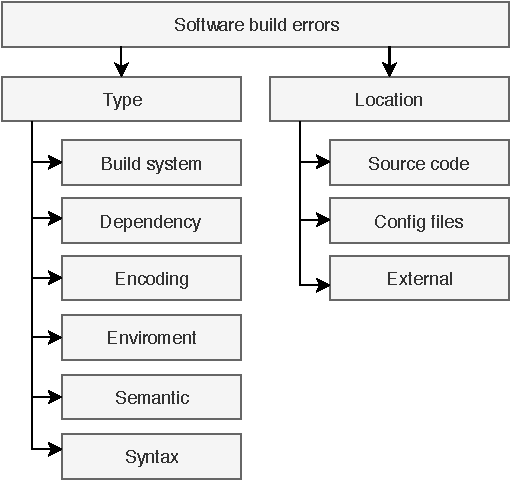
\includegraphics[width=11cm]{img/Taxonomy}
% 		\caption{Developed taxonomy of software build errors}
% 		\label{fig:taxonomyTree}
% 	\end{center}
% \end{figure}

\begin{table*}
	\caption{Taxonomy results}
	\label{table:taxonomyResults}
	\centering
	\begin{tabular}{>{\rowmac}r>{\rowmac}r>{\rowmac}r>{\rowmac}r>{\rowmac}r>{\rowmac}r>{\rowmac}r>{\rowmac}r<{\clearrow}}
		\setrow{\bfseries} & CLOSURE & LANG    & MATH    & MOCKITO & SPRING  & TIME     & Average \\
		\toprule
		\setrow{\bfseries}
		Build system & 33.33\% & 91.15\% & 94.41\% & 98.62\% & 61.18\% & 100.00\% & 79.78\%        \\
		\midrule
		Config Files & 0.00\%  & 0.06\%  & 0.00\%  & 21.42\% & 1.93\%  & 0.00\%   & 3.90\%         \\
		External     & 33.33\% & 91.09\% & 94.41\% & 77.20\% & 59.25\% & 100.00\% & 75.88\%        \\
		\midrule
		\setrow{\bfseries}
		Dependency   & 33.33\% & 0.30\%  & 0.00\%  & 0.95\%  & 9.55\%  & 0.00\%   & 7.36\%         \\
		\midrule
		Config Files & 0.00\%  & 0.30\%  & 0.00\%  & 0.67\%  & 5.69\%  & 0.00\%   & 1.11\%         \\
		External     & 0.00\%  & 0.00\%  & 0.00\%  & 0.00\%  & 0.36\%  & 0.00\%   & 0.06\%         \\
		Source Code  & 33.33\% & 0.00\%  & 0.00\%  & 0.29\%  & 3.50\%  & 0.00\%   & 6.19\%         \\
		\midrule
		\setrow{\bfseries}
		Encoding     & 0.00\%  & 6.58\%  & 0.00\%  & 0.00\%  & 1.78\%  & 0.00\%   & 1.39\%         \\
		\midrule
		Source Code  & 0.00\%  & 6.58\%  & 0.00\%  & 0.00\%  & 1.78\%  & 0.00\%   & 1.39\%         \\
		\midrule
		\setrow{\bfseries}
		Enviroment   & 0.00\%  & 0.00\%  & 0.00\%  & 0.00\%  & 20.70\% & 0.00\%   & 3.45\%        \\
		\midrule
		External     & 0.00\%  & 0.00\%  & 0.00\%  & 0.00\%  & 20.70\% & 0.00\%   & 3.45\%        \\
		\midrule
		\setrow{\bfseries}
		Semantic     & 33.33\% & 1.85\%  & 5.59\%  & 0.43\%  & 6.78\%  & 0.00\%   & 8.00\%         \\
		\midrule
		Source Code  & 33.33\% & 1.85\%  & 5.59\%  & 0.43\%  & 6.78\%  & 0.00\%   & 8.00\%         \\
		\midrule 
		\setrow{\bfseries}
		Syntax       & 0.00\%  & 0.12\%  & 0.00\%  & 0.00\%  & 0.02\%  & 0.00\%   & 0.02\%         \\
		\midrule
		Config Files & 0.00\%  & 0.06\%  & 0.00\%  & 0.00\%  & 0.00\%  & 0.00\%   & 0.01\%         \\
		Source Code  & 0.00\%  & 0.06\%  & 0.00\%  & 0.00\%  & 0.02\%  & 0.00\%   & 0.02\%        
	\end{tabular}
\end{table*}

\vspace{0.3cm}
\begin{tcolorbox}[fonttitle=\bfseries,title=Answer to RQ2: What are the most common problems that cause
	snapshot build fail?,label=rq2,colframe=blue!50!black]
	Considering the taxonomy made and the errors classified in it, we can conclude that the most common errors we find when building the snapshot of a Java project are due to the Build System (79.78\%), to the semantics of the language (8.00\%) and to the dependencies of the project (7.36\%). Other less common errors are related to the environment (3.45\%), encoding (1.39\%) and syntax (0.02\%).
\end{tcolorbox}


\chapter{Discussion}
\label{sec:discussion}
This section discusses implications of the experimental results, the observations from our study on buildability and the proposed taxonomy, followed by an approximation of mitigation measures. In addition, it discusses limitations and threats to validity.

\section{Implications of experimental results}

First, we expected the projects to have a stable build history (all of them are Open Source libraries), with some points in the past where the project could not be built. This idea has only materialized in the Closure project. In the rest of the projects we have found a common problem, a change in the build system of the project, which considerably reduces the number of buildable commits. The main disadvantage of pre-setting the construction system and assuming that it will not vary significantly affects the study, but at the same time gives us valuable information about the evolution of the projects and how we must adapt.

Running the experimentation required a significant investment of time and resources. It was necessary to run the experiment on isolated machines (one per project) that were running for several days sequentially executing the builds of each project. Some measures to mitigate the amount of time required were the elimination of tasks at build process that did not directly affected the project, such as the generation of automatic documentation or the execution of tests, which was not considered within the scope of the experiment. In some projects, as in the case of Spring Framework, there was the problem of Maven Central (from where dependencies are downloaded) banning the IP of the machine as a result of an abuse of the API, that externally prevented the correct build of the project, having to limit the number of builds per time to avoid it.

\section{Implications of proposed taxonomy}

The taxonomy developed in this work proposes a high-level classification easily extensible that collects the types of errors and their location in the project. The taxonomy was intended to be an answer to RQ2, but we found that this is only one dimension within the most exhaustive classification that can be carried out. We introduce the dimension of the location of the error (in which place of the project it occurs -- or if it occurs outside of it-- ). Other dimensions not included but possible could be the involvement of the developer (complex in some cases due to the lack of knowledge of the development phase) in the error or the difficulty of its solution (it can be subjective).

Most of the problems we find in the construction of a project are not affected by the compilability of the project, so they would be extendable to the scope of dynamic languages

%Providing a categorization of errors empirically is not easy. We must leave any preconceived ideas of what the problems will be like to stick only to the results. Initially, we found all built problems unclassified, we only knew where were they localized in the history of commits. By grouping together problems related to consecutive commits we found that usually the build failures were produced by the same problem. Once grouped, it was enough to choose a failed build, check its log and extract the pattern that identified it to apply it again to all the failed builds. This process was repeated until there was no unclassified failed builds. The patterns had to be generic enough to be able to capture different variants of the same error, but in some cases it was necessary to particularize the error in order to get the specific classification.

%Common patterns were found for the different Java projects, independent of the build system used, such as

%\begin{lstlisting}
%	error: (.+)\n(.+)
%\end{lstlisting}

%which classifies the errors derived from the compilation of Java code and in turn allows subcategories based on their variants, for example

%\begin{lstlisting}
%	error: incompatible types
%\end{lstlisting}

%These cases strengthen our choice of Java as a technology on which to investigate buildability: the structured logs provided by the compiler and build systems allowed us to make a simple and automated tracking of errors.

\section{Mitigation measures}

While we were doing the taxonomy, we realize that some of the problems we encountered could be easily solved to achieve a successful build and others were more complicated or unfeasible.

Some generic solutions, that requires changes in the configuration or in the command launched by the project but not in the source code itself, follows:

\begin{itemize}
	\item \textbf{Build system change} Detect which technology is being used to build the project to use the most convenient one in each case (search pom.xml for Maven, build.xml for Ant, etc).
	\item \textbf{Encoding problem} If it does not exist, add the property encoding in the project configuration file.
	\item \textbf{Dependency problem} If a dependency is a SNAPSHOT, look for the compatible version that is stable and recoverable from the dependency repository. Replace this dependency with the stable one in the configuration before executing the build.
	\item \textbf{Environment problem} Check the resource requirements of the project.
\end{itemize}

For the following problems, the solution is usually not trivial or cannot easily be automated:

\begin{itemize}
	\item \textbf{Java compilation issue: Syntax and semantic} Requires modification of the source code of the project.
	\item \textbf{Build configuration issues} Requires a deep knowledge of how the project is built.
\end{itemize}

These problems are usually specific code errors that do not affect too many versions, because the developers often correct them quickly.

\section{Limitations and Threats to Validity}

The validity of our work is described in terms of the four main threats to validity in empirical software engineering research: construct, internal and external validity~\cite{Wohlin2012} (excluding statistical conclusion validity that does not apply to our problem).

% Construct validity: Does the treatment correspond to the actual cause we are interested in? Does the outcome correspond to the effect we are interested in?

\textbf{Construct validity} 
The results of the analysis corresponding to the RQ1 are affected essentially by the construction system of the project, so that a large number of fail builds of the projects may be hiding other causes of errors. We believe that an undocumented change in the way the project is built is a cause of error in itself.

%\hspace{5px}

% Internal validity: Did the treatment/change we introduced cause the effect on the outcome? Can other factors also have had an effect?

\textbf{Internal validity} Threats to internal validity relate to the experimenter; taxonomy has been made from empirical data (the logs of the failure builds) under the interpretation of a single researcher who performed the analysis. On the other hand, a well-documented taxonomy methodology has been used along with conceptual approaches in some of the iterations, specifically using in one of them the previous knowledge of taxonomy of errors in Java projects from another work.

%\hspace{5px}

% External validity, Transferability Is the cause and effect relationship we have shown valid in other situations? Can we generalize our results? Do the results apply in other contexts?

%\noindent
\textbf{External validity} A general threat to external validity is the representativeness of the selected subjects. In this study we use open source projects, which could not be representative of other software projects. However, we think we took this issue into consideration by including the Spring Framework project, which is a huge project heavily used in the industry, which is a good representative of a big project. 

% Conclusion validity: Does the treatment/change we introduced have a statistically significant effect on the outcome we measure?

%\textbf{Conclusion validity}  

%\grex{Include a sentence about construct and conclusion validity (related to how sure the conclusions reached in regards to the relationships in our data are reasonable.)}








\chapter{Conclusions and future Work}
\label{sec:conclusions}
This chapter recapitulates the initial objectives of the research and the contributions claimed in Chapter~\ref{chapter:intro}, in addition to presenting the conclusions (Section~\ref{sec:conclusions}) of the three studies included in this PhD. Thesis. 
In addition, Section~\ref{sec:future-work} also details future research work.

\section{Conclusions}
\label{sec:conclusions}

\subsection{Revisiting the building of past snapshots}

In Chapter~\ref{chapter:buildability} we have shown a replication and a reproduction study from Tufano et al. work~\cite{tufano2017there} about the compilability of the history of past commits of a project. 
In the first one we have repeated their analysis, with those repositories for which we found all commits, and in the second one we extended its generality by using the same methodology with a different, more diverse set of Java projects, and considering also Ant and Gradle in addition to Maven.

The main contributions of this chapter are:

\begin{itemize}
\item A discussion and guidelines on reproduction packages for studies on the compilability of past snapshots. 
\item A dataset and software, usable by other researchers, to study long-term degradation of compilability.
\item A partial validation of the results of the original study. In particular, results about frequency of errors causing build failures have been validated and extended.
\item Evidence on how compilability degrades over time, and how it could be mitigated by ensuring future availability of dependencies.
\item Evidence on the compilability of a different, more diverse set of Java projects, showing some differences with the original study.
\item Evidence on how the building tools affect future compilability.
\end{itemize}

%\grex{Lo he dejado así}
%:\jgb{Lo he retocado un poco}
In summary, we wanted to shed some more light on to which extent past snapshots of projects are compilable ``as such'', because that is the basis to know how much build-repair techniques are needed if past artifacts of a project need to be reproduced from source code.
Since our study was a replication and a reproduction, a part of our results could be expected, but still they add more detail and evidence to the original study. In addition, we also found some differences, generalized evidence by analyzing a more diverse set of projects, and produced a tool to automate the analysis of any Java repository, which could be used in further studies by any researcher.

\subsection{Running tests in past snapshots: an empirical study}

In Chapter~\ref{chapter:testability} we have started a path to analyze to which extent past snapshots of a project can be tested. 
For that, we have conducted an empirical analysis of many Java projects from a well-known dataset. 
We also propose a framework for conducting further analysis, based on the different steps needed to successfully run tests for each snapshot. 
Using this framework, we have found that for more than half the snapshots, all tests cannot be run successfully.
However, the main result is the high variability of testability from project to project, even within relatively homogeneous dataset. 
% In this respect, we also discard some hypothesis on the influence of characteristics of projects (lines of code, number of commits, age) in testability.

%In this paper we offer a study of the testability of the history of 111 Java projects, which extends previous studies on the buildability of project history. 
%We also provide a complete study that discards some of the most common metrics of a project (lines of code, number of commits or its age) as factors that determine its testability. 
%We have found that in most projects it is not possible to reproduce the tests in the past.
%In addition, we conducted a preliminary study of the causes that can lead to low testability in Java projects.
%Analysing the projects we have found great variability, even among projects selected under the same criteria. 

We note that many projects cannot rely on running tests in past commits, as these won’t run or even compile.
Testing snapshots of the past is fundamental for the maintainability of old versions of the project which are still in production. 
Therefore, we expect more research in this area in the future. 
% Fortunately, we have found some signals showing that good practices can be identified to increment testability of current snapshots (that will become past snapshots with time). 
We have also suggested some ways of increasing testability of past snapshots improving the methods we are using for building and running tests in them. 
Of course, extending our study to other samples of Java code, and to other programming languages, will improve our knowledge in this area.

%and also that some techniques could be used to of those snapshots, 
%Replication testing is essential to improve the maintainability of projects that need to be maintained in previous versions.
%Reproducing this study using other languages such as Python, Javascript or C++ could lead to interesting future work.

\subsection{Bug localization trough regression testing}

In Chapter~\ref{chapter:bug-hunter} we leverage the knowledge and tools researched in Chapters~\ref{chapter:buildability} and~\ref{chapter:testability} to operationalize the theoretical method, called \emph{perfect test}, to detect the change that introduced a bug (BIC), by using a regression test as perfect test. We show, using a well-known bugs dataset~\cite{just2014defects4j}, that the method works for those bugs where we are able to transplant the regression test in the past and find a commit where this test passes again, by using our tool to automatically detect the BIC and then validating the results. 

However, we also find that our method is limited by the transplantability of regression tests to past snapshots, and in particular by the compilability of past snapshots.

As a result of applying our method, we produce, by a completely automated procedure, a dataset of BICs (\datasetName), that can be used as ground truth for evaluating methods for detecting BICs. 
We apply it to some SZZ derivatives, proposing a method for evaluating their relative performance, and verifying a well-known limitation of them. 
This method could be exploited for producing, automatically, much larger collections of BICs. 
We also propose our method for automatically providing developers fixing a bug with detailed information about the BIC that introduced it.

\section{Future Work}
\label{sec:future-work}

The studies presented in this PhD. Thesis are limited to projects written in the Java programming language. Moreover, these projects are mostly programming libraries, which usually have only unit tests and sometimes integration tests.
Therefore, further research is still needed to draw general conclusions on the compilability of past snapshots, testability of the past snapshots and to identify the change that introduced the bug, especially for languages other than Java (C, C++, Python, JavaScript, Go, Rust and other popular programming languages), and in general to projects with different testing practices (e.g., including load testing or end-to-end testing).

In Chapter~\ref{chapter:testability}, one of the main limitations we have encountered when running the tests is to reproduce in context the test execution. Despite having the tests collected in the commit history, we do not have the information of whether these tests could be compiled and subsequently executed, as well as the absence of the result of the execution. 
This information could be obtained from the Continuous Integration (CI) system (if used), where the build of projects and the execution of their tests is done automatically, and their results are recorded.
It has been a very common practice for open-source projects to use continuous integration systems that are not publicly accessible (such as Jenkins) and therefore it is not possible to retrieve test building and execution information. 
Even so, many projects have used Travis~\footnote{\url{https://www.travis-ci.com/}} as a continuous integration system. This CI system has allowed projects such as TravisTorrent~\cite{msr17challenge} to offer build and test execution datasets for over 1,000 projects. 
Within the open-source world, this CI system is gradually being replaced by GitHub Actions, another CI system integrated into the GitHub platform (the most widely used Git repository platform). 
Therefore, a possible future work would be to create a new dataset of builds and test executions to help us understand how the tests behaved at the time they were executed and in the right context. 
This future work would have to deal with problems such as the fact that such executions (together with their results and logs) usually have a maximum lifetime of 90 days, so we would have to "record" such executions over a period of time.

In Chapter~\ref{chapter:bug-hunter}, we propose a tool that exhaustively searches for the change that introduced an error. 
However, this tool is limited by the problems in reproducing the test context and the time required to compute the regression test run results in the change history.
It would be interesting to continue the proposed work by trying to combine our tool with the most recent implementations of SZZ. 
Our tool would refine and extend the candidates proposed by this algorithm, while the SZZ algorithm could sensibly reduce the execution time of our tool by filtering out irrelevant changes.

% The replication and reproduction study in Chapter~\ref{chapter:buildability} continues the work of Tufano et al.~\cite{tufano2017there}, validating and extending its conclusions. 
% However, both studies and remain very limited to the Java programming language, but also to projects that are basically programming libraries. 
% Future lines of work can extend this study by exploring the application of the method on datasets of projects in other programming languages than Java (Python, C, C++ ...), of other types of projects (not only libraries), and in general to projects with different testing practices.

% Ap-ndices
%\appendix
%\include{...}
%\include{...}
%\include{...}

\backmatter

%
% Bibliography
%

%%---------------------------------------------------------------------
%
%                      configBibliografia.tex
%
%---------------------------------------------------------------------

%%%%%%%%%%%%%%%%%%%%%%%%%%%%%%%%%%%%%%%%%%%%%%%%%%%%%%%%%%%%%%%%%%%%%%
% Definici-n de los ficheros .bib utilizados:
% \setBibFiles{<lista ficheros sin extension, separados por comas>}
% Nota:
% Es IMPORTANTE que los ficheros estén en la misma l-nea que
% el comando \setBibFiles. Si se desea utilizar varias l-neas,
% terminarlas con una apertura de comentario.
%%%%%%%%%%%%%%%%%%%%%%%%%%%%%%%%%%%%%%%%%%%%%%%%%%%%%%%%%%%%%%%%%%%%%%
\setBibFiles{%
bibliography%
}

\setCitaBibliografia{
\begin{FraseCelebre}
\begin{Frase}
  If I have seen further than others, it is by standing upon the shoulders of giants
\end{Frase}
\begin{Fuente}
  Isaac Newton
\end{Fuente}
\end{FraseCelebre}
}

%%
%% Creamos la bibliografia
%%
\makeBib

% Variable local para emacs, para  que encuentre el fichero maestro de
% compilaci-n y funcionen mejor algunas teclas r-pidas de AucTeX

%%%
%%% Local Variables:
%%% mode: latex
%%% TeX-master: "../Tesis.tex"
%%% End:


\specialHead{Bibliography}
\bibliographystyle{abbrv}
\bibliography{bibliography}

%
% Final
%
\ifpdf
   \pdfbookmark{Fin}{fin}
\fi

\thispagestyle{empty}\mbox{}

\vspace*{4cm}

\small

\hfill \emph{Part of the journey is the end -- Tony Stark --}

\newpage


\end{document}
